\documentclass[11pt,a4paper]{article}

\usepackage[T1]{fontenc}
\usepackage[utf8]{inputenc}
\usepackage{lmodern}
\usepackage[margin=2.2cm]{geometry}
\usepackage{graphicx}
\usepackage{booktabs}
\usepackage{siunitx}
\usepackage{amsmath,amssymb}
\usepackage{caption}
\usepackage{subcaption}
\usepackage{tikz}
\usetikzlibrary{arrows.meta,positioning,fit}
\usepackage{xcolor}
\usepackage{float}
\usepackage[hidelinks]{hyperref}

\sisetup{detect-all}
\setlength{\emergencystretch}{2em}
\captionsetup{font=small,labelfont=bf}
\graphicspath{{figures/}}

\title{Background-Sector Phase-Space Sampling for the DCS-Monitor\\[2pt]
\large 64-Cell Pilot and HPC Validation Plan}
\author{DCS-Monitor simulation notes}
\date{\today}

\begin{document}

\maketitle

\begin{abstract}
The DCS-Monitor simulation must estimate the detector response to radiation
originating in neighbouring spent-fuel casks, not only in the target cask. A
direct full-array transport calculation is unnecessarily expensive because the
same cask-to-sector phase space is reused for many detector and shield
configurations. This report describes a two-stage factorised workflow: a
pilot-scale \texttt{p1.5} production step scores the first entry of each gamma
or neutron into a 64-cell shell around the target cask, and a
\texttt{p2\_bkgd} replay step transports those unit-weight entries through the
detector geometry. The shell is divided into eight azimuthal sectors and eight
longitudinal layers spanning the cask height from \SI{-2040}{mm} to
\SI{+2040}{mm}. It lives in a Geant4 parallel world, so it has no material and
does not alter the mass geometry. The replay deduplicates entries by source
event: for each source event it keeps the entry with the earliest global time,
then the smaller cell identifier. This removes repeated crossings of the
artificial cell boundaries, but it also retains only one candidate entry per
event, so it is an approximation rather than a track-level transport of every
crossing. A \SI{662}{keV} gamma check against a direct ZLN calculation for cask
4 and global fuel 0 gives 961 detector hits and \SI{208.740}{MeV} in the
64-cell two-cell replay, compared with 1003 hits and \SI{209.756}{MeV} from the
direct ZLN result scaled from \SI{180}{s} to \SI{36}{s}. The test contains
about 953 independent hit events, so the ratios of 0.958 in hit count and 0.995
in deposited energy are consistent with the direct result at the approximately
3\% statistical level. A four-cell variant gives 1016 hits and
\SI{212.392}{MeV}, bracketing the direct yield. The report also sets out the
production matrix, merging requirements, and the HPC validation plan needed for
a physics result.
\end{abstract}

\tableofcontents

\section{Motivation and scope}

The nominal DCS-Monitor simulation starts from the target cask and follows
radiation through the cask body, the detector shield, and the detector. That
approach is appropriate for the target cask, but the detector also sees
radiation produced in the other eleven casks in the storage hall. Repeating the
full source-to-detector transport for every neighbouring cask, hexant, detector
position, and shield variant would multiply the cost by the number of
configurations.

The workflow in this report factorises the problem at a fixed geometric
surface. The expensive cask-to-surface transport is performed once per source
configuration, and the resulting phase space is reused for the cheaper
surface-to-detector transport. The factorisation is exact only in the sense of
phase-space sampling: it assumes that a recorded entry is upstream of the
detector for the relevant particles and that the shell encloses the detector and
shield volume. The event-level deduplication described in
Section~\ref{sec:replay} is a second approximation. Both assumptions are part
of the validation plan.

This report is deliberately a pilot report. The numerical results use one gamma
line, one source cask, and a one-million-event subset of the source file. They
demonstrate that the implementation and the bookkeeping are consistent; they are
not a final background estimate.

\section{Geometry and source model}

\subsection{Storage hall and detector positions}

The hall contains twelve CASTOR~440/84 casks arranged as three clusters: a
central $2\times2$ group and two four-cask side groups. The target cask is cask
0 at $(x,y)=(\SI{1580}{mm},\SI{1580}{mm})$. The concrete floor and the two side
walls are included in the mass geometry. The detector scan uses eight positions
at $45^\circ$ intervals, nominal radius \SI{1350}{mm}, and $z=\SI{150}{mm}$.
The hemi-shield variant uses a larger effective radius of about
\SI{1445}{mm}. Figure~\ref{fig:hall} shows the plan view and the relation between
the hall, the cask array, the detector positions, and the scoring shell.

\begin{figure}[t]
  \centering
  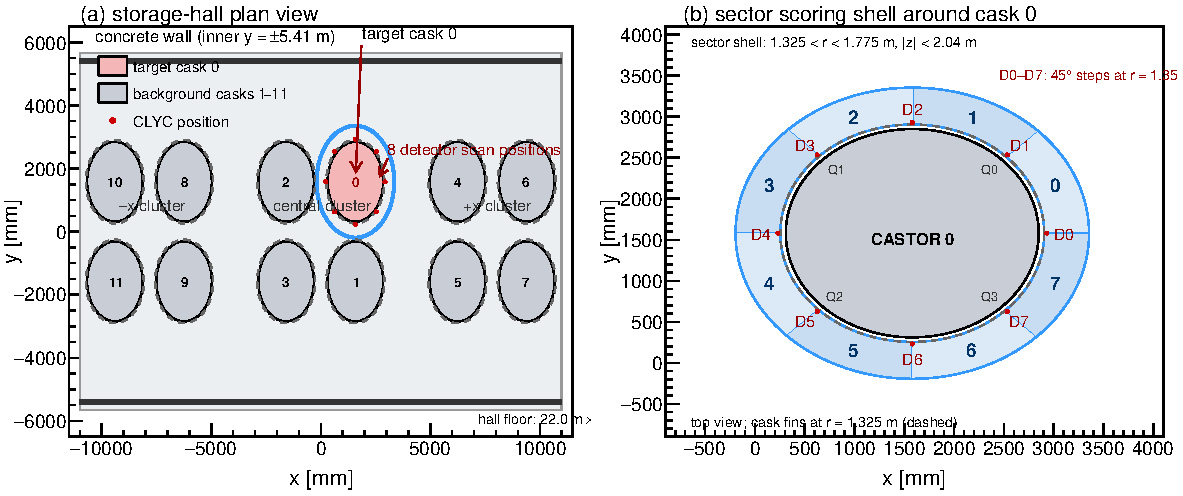
\includegraphics[width=\linewidth]{fig_hall_sectors.pdf}
  \caption{Storage-hall plan view (left) and the 64-cell scoring shell around
  target cask 0 (right). The shell is drawn in the cask-local frame; it is a
  scoring surface, not a material volume. The detector positions D0--D7 are
  shown at their nominal \SI{1350}{mm} radius inside the shell.}
  \label{fig:hall}
\end{figure}

\subsection{The 64-cell scoring shell}

The shell is divided into eight non-overlapping \ang{45} azimuthal sectors and
eight longitudinal layers. Its inner radius is \SI{1325}{mm}, just outside the
fin tips of the CASTOR body; its outer radius is \SI{1775}{mm}; and its
longitudinal extent is \SI{-2040}{mm} to \SI{+2040}{mm}, in the target-cask
frame. The eight layers therefore have a thickness of \SI{510}{mm}. The
parameters are collected in Table~\ref{tab:geometry}. The shell lives in the
\texttt{SectorScoringWorld} parallel world and therefore has no material. It
changes neither the transport nor the detector response.

The cell identifier is
\begin{equation}
  \texttt{cellId} = \texttt{zLayer}\times 8 + \texttt{sector},
  \label{eq:cellid}
\end{equation}
so the first eight identifiers are the eight azimuthal sectors of the bottom
layer and the last eight are those of the top layer. A detector at
$z=\SI{150}{mm}$ lies in layer 4, which covers $z=\SI{0}{mm}$ to
\SI{510}{mm}. The nominal detector at $\varphi=0^\circ$ lies on the boundary
between sectors 0 and 7, so the automatic cell selection described in
Section~\ref{sec:replay} returns both sector cells in layer 4: cell 32 and cell
39.

\begin{table}[t]
  \centering
  \caption{Reference geometry used by the 64-cell sector scoring and the
  \SI{662}{keV} gamma validation.}
  \label{tab:geometry}
  \begin{tabular}{@{}lll@{}}
    \toprule
    Quantity & Value & Note \\
    \midrule
    Casks in hall & 12 & three clusters of four \\
    Target cask position & $(\SI{1580}{mm},\SI{1580}{mm})$ & cask 0 \\
    Cask body outer radius & \SI{1270}{mm} & fin-tip radius $\approx\SI{1325}{mm}$ \\
    Sector inner radius & \SI{1325}{mm} & at the fin tips \\
    Sector outer radius & \SI{1775}{mm} & encloses the detector at \SI{1350}{mm} \\
    Sector $z$ extent & \SI{-2040}{mm} to \SI{+2040}{mm} & cask height \\
    Azimuthal sectors & 8 & \ang{45} each, non-overlapping \\
    Longitudinal layers & 8 & \SI{510}{mm} each \\
    Scoring cells & 64 & $\texttt{zLayer}\times 8+\texttt{sector}$ \\
    Entry faces per cell & 6 & inner, outer, two caps, two sides \\
    Detector scan radius & \SI{1350}{mm} & nominal, $z=\SI{150}{mm}$ \\
    Hemi-shield effective radius & $\approx\SI{1445}{mm}$ & for the shield variant \\
    \bottomrule
  \end{tabular}
\end{table}

Each first entry is assigned to one of the six boundary faces by the smallest
distance to the inner cylinder, the outer cylinder, the top cap, the bottom cap,
or one of the two azimuthal side planes. Faces 0--3 are the cylindrical and cap
surfaces; faces 4 and 5 are the lower- and upper-$\varphi$ side faces of the
cell. For cells that are not at the bottom or top of the shell, the two
longitudinal faces are internal boundaries shared with the adjacent layer; they
are labelled 6 and 7 so that they can be separated from the two external caps.
The face label is not used in the transport. It is used to verify that the shell
is populated through all expected surfaces and to diagnose boundary duplicates.

Figure~\ref{fig:rz} shows the radial--longitudinal cross-section. The shell
encloses the detector: the inner face is just outside the cask at
\SI{1325}{mm}, the detector sits at the nominal \SI{1350}{mm} scan radius, and
the outer face is at \SI{1775}{mm}. Inner-face entries are therefore upstream of
the detector, while outer, top, and bottom entries are particles entering from
the surrounding hall. The two azimuthal side faces carry particles crossing
between neighbouring sectors; they are retained as local boundary sources for
the replay. The shell now spans the full cask height, so the cask top and bottom
are not truncated by the scoring surface. The eight longitudinal layers localise
an entry to a \SI{510}{mm} interval and prevent a single cell from covering both
the detector and the cask ends.

\begin{figure}[t]
  \centering
  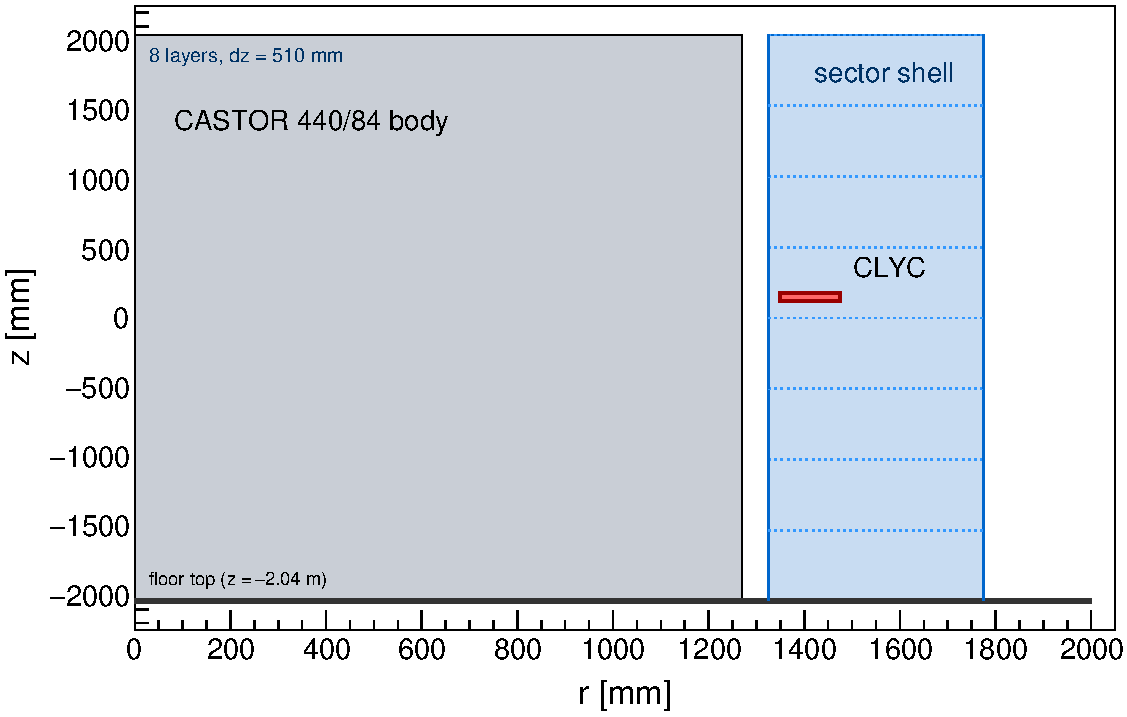
\includegraphics[width=0.78\linewidth]{fig_sector_rz.pdf}
  \caption{Radial--longitudinal view of the target cask, the 64-cell scoring
  shell ($\SI{1325}{mm}<r<\SI{1775}{mm}$, $\SI{-2040}{mm}<z<\SI{2040}{mm}$),
  and the detector at $z=\SI{150}{mm}$. The horizontal dashed lines mark the
  eight \SI{510}{mm} layers. The shell is a parallel-world scoring volume.}
  \label{fig:rz}
\end{figure}

\subsection{Visual check of the array}

The OpenGL views in Figure~\ref{fig:ogl} are a quick geometric check of the
twelve-cask array and the target detector position. The hall is omitted in
these renders so that the cask bodies are not obscured by the semi-transparent
walls; the hall outline is shown in Figure~\ref{fig:hall}. Internal cask details
are hidden in the renders to keep the exported vector files manageable. These
images are illustrative, not a substitute for the dimensioned plan view.

\begin{figure}[t]
  \centering
  \begin{subfigure}[t]{0.48\linewidth}
    \centering
    
\includegraphics[width=\linewidth]{fig_ogl_top.pdf}
    \caption{Top view of the twelve casks.}
  \end{subfigure}\hfill
  \begin{subfigure}[t]{0.48\linewidth}
    \centering
    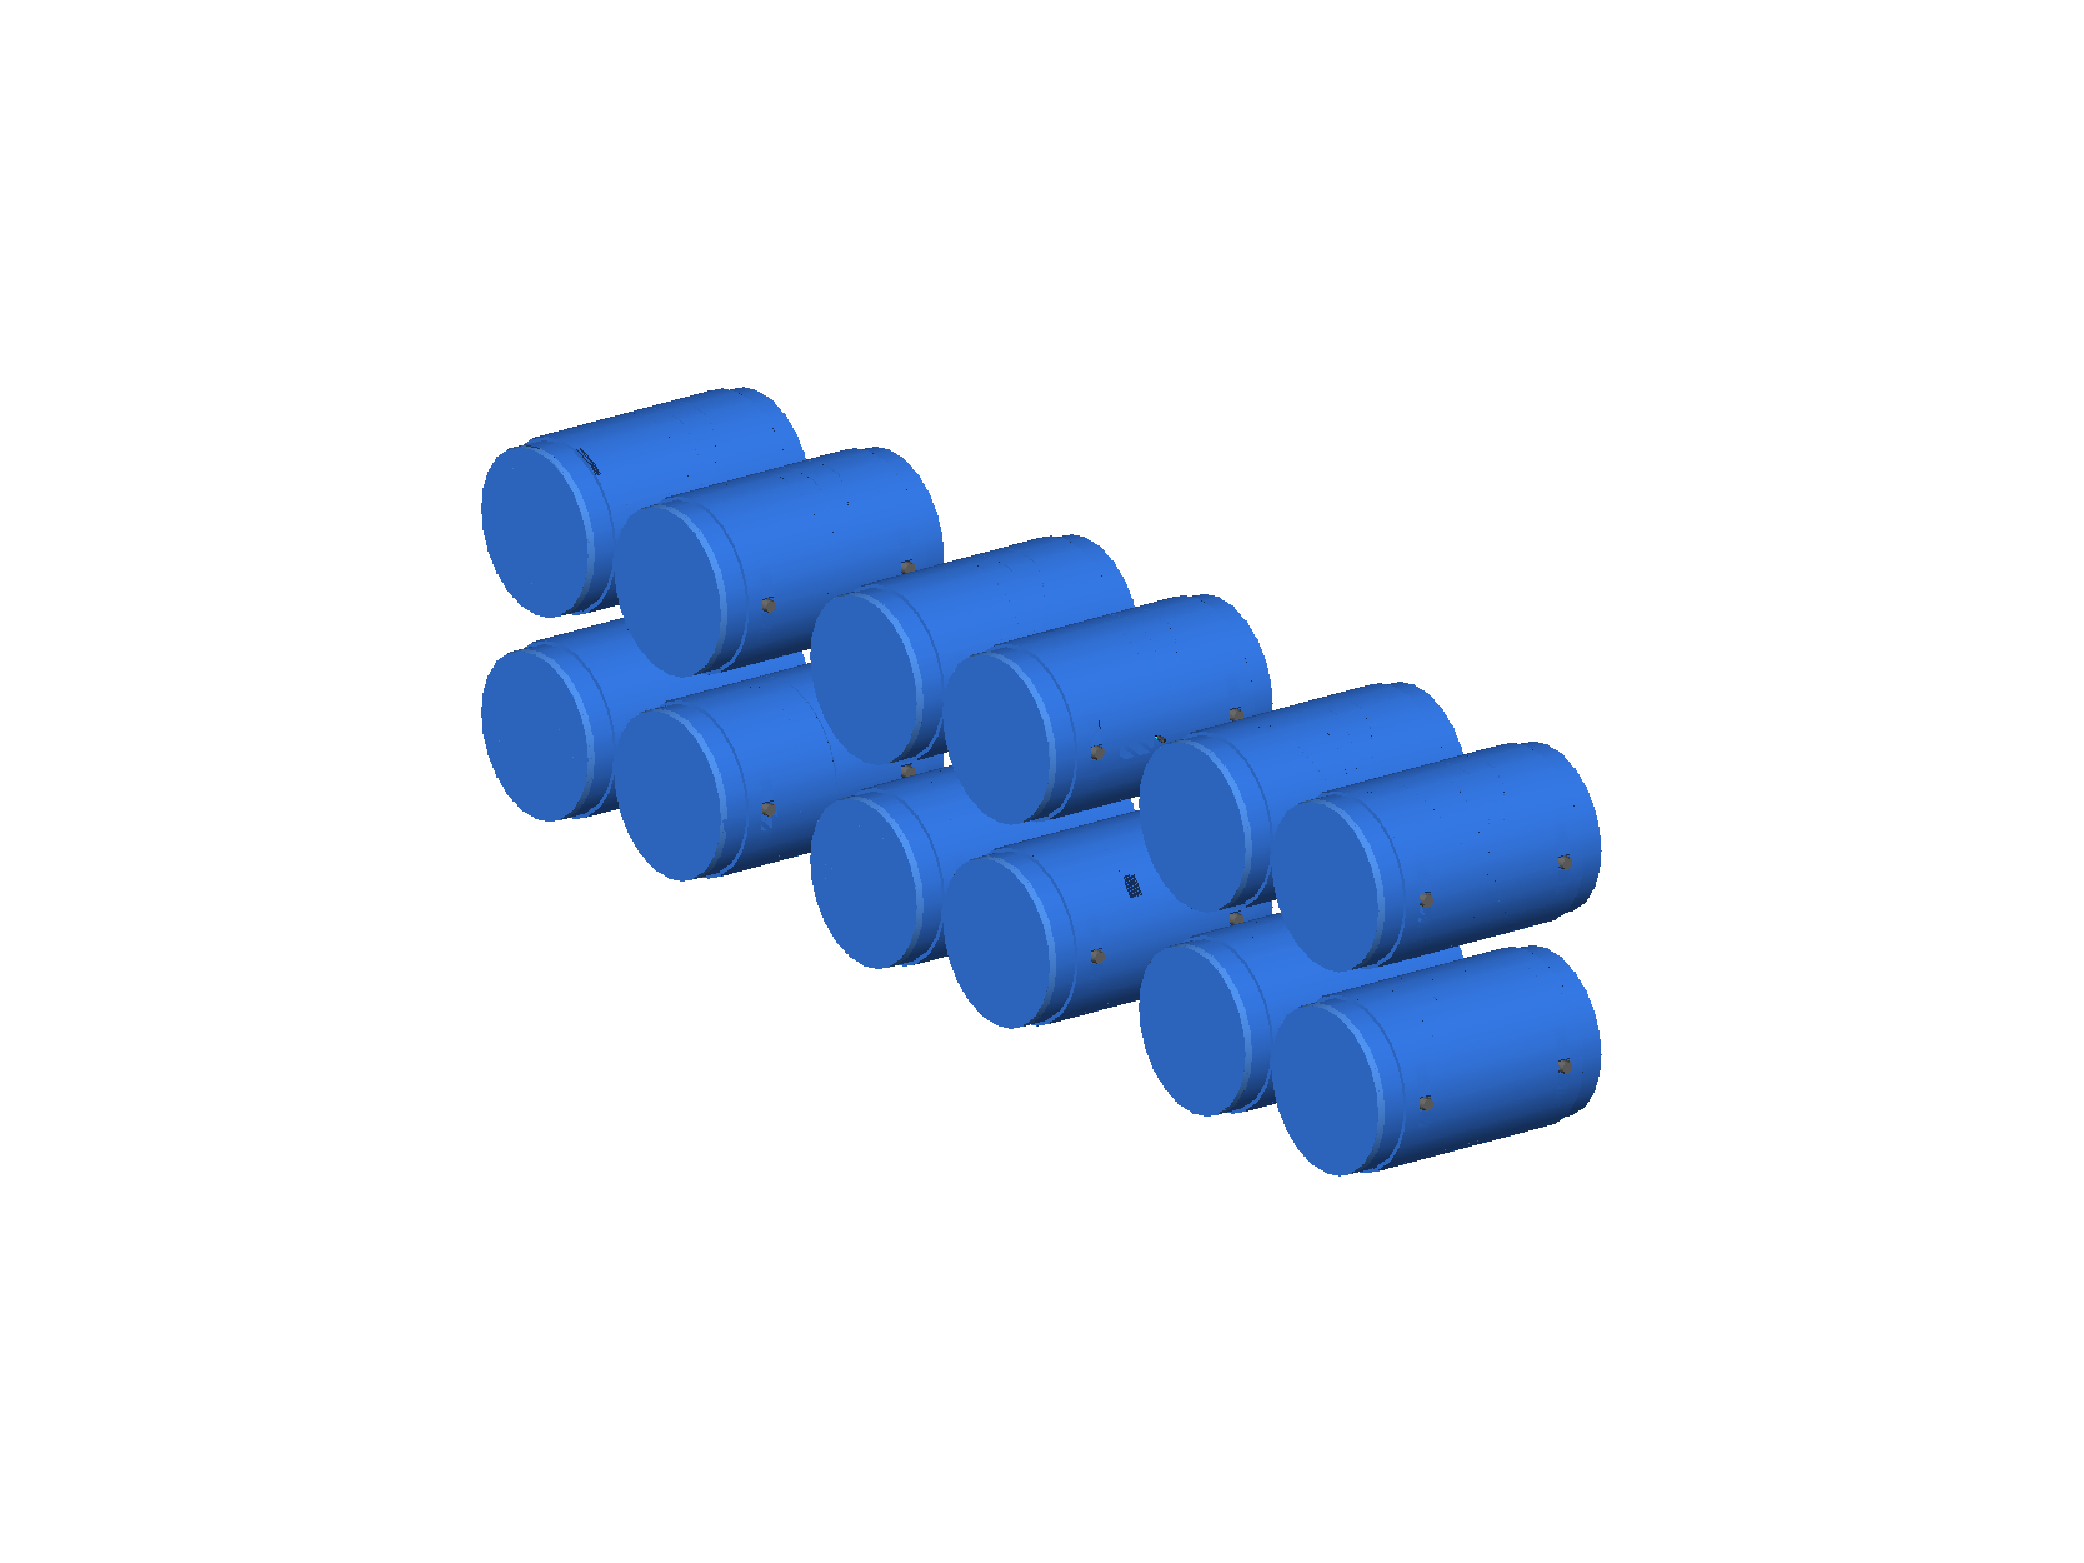
\includegraphics[width=\linewidth]{fig_ogl_oblique.pdf}
    \caption{Oblique view.}
  \end{subfigure}
  \caption{Geant4/OpenGL renders of the cask array with the target detector
  included. The hall is hidden for clarity. The top view shows the six cask
  columns (two rows); the oblique view shows the three clusters in perspective.}
  \label{fig:ogl}
\end{figure}

\subsection{From p1 surface flux to p1.5 sector flux}

The existing p1 stage records particles crossing the outer surface of a cask.
Each entry contains the particle type, kinetic energy, position, direction, and
the statistical weight from the original source calculation. The p1.5 stage
samples those crossings, applies the same surface smearing as the nominal p2
workflow, and transports the resulting particles in a geometry that contains all
twelve casks but no detector. The 64-cell shell records the first entry of each
gamma or neutron into each cell.

For a p1 file with $N_{p1}$ generated primaries and total kept weight
$W_{\mathrm{kept}}$, the weight ratio is
\begin{equation}
  r=\frac{W_{\mathrm{kept}}}{N_{p1}}.
\end{equation}
For a requested generation time $T_{\mathrm{gen}}$ and a source decay rate
$\lambda$, the p1.5 driver computes
\begin{equation}
  N_{p1.5}=\lambda\,T_{\mathrm{gen}}\,r,
  \label{eq:nps}
\end{equation}
clamped to the \texttt{/run/beamOn} ceiling when necessary. The value of
\texttt{numPrimaries} sets the number of source events read from the p1 file; it
does not set the number of events that reach the shell. The output
\texttt{sectorFlux} tree has $M$ entries for a run. Each entry is stored with
unit weight because the p1 weights have already been folded into the sampling.
The provenance is written once to the \texttt{sectorMeta} tree:
$T_{\mathrm{gen}}$, $M$, $N_{p1.5}$, $r$, the source cask, the hexant, the
source type, the target cask, the shell dimensions, the number of azimuthal
sectors, the number of longitudinal layers, and the number of cells.

The important bookkeeping rule is that $M$ is the total number of
\texttt{sectorFlux} entries in the file, not a per-cell count. A single p1.5 run
therefore writes one metadata row whose $M$ is the sum over the cells that were
populated. A merged production file must either carry one row per cell or add an
explicit per-cell count; the replay sampler computes the filtered count
$M_{\mathrm{loaded}}$ and the deduplicated count $M_{\mathrm{unique}}$ for the
requested cell selection.

\section{Implementation}

\subsection{Parallel world and first-entry scoring}

The scoring geometry is a \texttt{G4VUserParallelWorld}. The mass geometry is
constructed first; the parallel world then places $8\times 8=64$ \texttt{G4Tubs}
cells at the target-cask position and orientation. Because the cells have no
material, they are invisible to the physics processes. The sensitive detector is
attached only to the parallel-world logical volumes.

A naive implementation would record every step inside a cell, which would count
a track many times and would make the entry multiplicity depend on the step
limiter. The implementation instead records the first entry of each track into
each cell. A thread-local registry maps the track identifier to a 256-bit mask.
When a track is created, it inherits its parent's mask; when it crosses a cell
boundary for the first time, the corresponding bit is set and the entry is
recorded. The track is not killed. This preserves the full shower and allows a
secondary produced in one cell to be counted when it later enters a different
cell.

Only gammas (PDG 22) and neutrons (PDG 2112) are recorded, matching the p1
surface-flux source. The step must have \texttt{fGeomBoundary} status, so a step
that merely starts inside a cell because of a geometry boundary is not mistaken
for a fresh entry. The recorded position is the pre-step point, and the
direction is the unit momentum at that point. The cell identifier is the copy
number of the parallel-world physical volume; the sector and longitudinal layer
are decoded with Equation~\eqref{eq:cellid}.

The scoring shell is registered only when the executable is started in
background-sector mode (\texttt{-{}-mode} \texttt{background-sector}). This is
not a convenience flag: the parallel world must be registered before the macro
executes, because the run manager builds the parallel geometry during
initialisation. The mode is analog, so combining it with \texttt{-{}-biasing} is
rejected.

\subsection{p1.5 production}

A p1.5 run uses the existing surface generator in
\texttt{CASTOR440\_surface\_from\_TTree} mode. The p1 source file is loaded once,
the requested cask and hexant are selected, the surface smearing is applied, and
the particles are transported through the full cask array. The detector and its
shield are absent. The output contains the \texttt{sectorFlux} tree and the
\texttt{sectorMeta} provenance row.

The validation macro sets \texttt{/dcs-monitor/det/setSectorZLayers 8} before
\texttt{/run/initialize}, loads the full one-million-event gamma subset, and
lets the decay rate and generation time determine the primary count. The target
cask is present but passive; the source cask is selected with
\texttt{/surf/caskNum}, and the hexant is selected with
\texttt{/surf/sourceRotZ}. The source type, global fuel index, and batch
identifier are copied into every entry and into the metadata.

\subsection{p2\_bkgd replay and event deduplication}
\label{sec:replay}

The replay source is a separate generator mode,
\texttt{BACKGROUND\_SECTOR\_from\_TTree}. It loads the \texttt{sectorFlux} tree,
optionally filters on cell identifier or longitudinal layer, and samples entries
uniformly. The sampler stores only the quantities needed by the generator: PID,
kinetic energy, time, position, and unit direction. The positions are already in
the global frame, so no cask translation or rotation is applied at replay time.

The cell filter can be given explicitly with
\texttt{/dcs-monitor/bkg/cellIds}, or it can be derived from the detector
geometry with \texttt{/dcs-monitor/bkg/autoCells true}. The automatic selection
builds the oriented detector envelope, transforms its corners into the
target-cask frame, and selects every cell whose radial, azimuthal, and
longitudinal intervals overlap the envelope. For the nominal CLYC assembly it
selects cells 32 and 39, the sector-0 and sector-7 cells of layer 4. The
inclusive layer overlap is deliberate: a detector that touches a layer boundary
must not lose entries from the adjacent layer.

The replay applies a per-event deduplication before sampling. The key is
\begin{equation}
  (\texttt{sourceKey},\texttt{evtNb}),
\end{equation}
where \texttt{sourceKey} packs the source cask, source type, hexant, global fuel,
and batch identifier, and \texttt{evtNb} is the p1.5 event number. For each key
the sampler keeps the entry with the smallest global time; if two entries have
the same time, it keeps the one with the smaller cell identifier. The counts are
reported as
\begin{equation}
  M_{\mathrm{loaded}} \ge M_{\mathrm{unique}} = M,
\end{equation}
where $M_{\mathrm{loaded}}$ is the number of entries after the cell filter and
before deduplication. For a replay of duration $T_{\mathrm{replay}}$, the number
of generated primaries is
\begin{equation}
  N_{\mathrm{replay}}=M_{\mathrm{unique}}\,
  \frac{T_{\mathrm{replay}}}{T_{\mathrm{gen}}}.
  \label{eq:replay}
\end{equation}
The replay sets the particle weight to one; it must not apply the p1 or p1.5
weight again.

The deduplication is not track-aware. A source event that enters two selected
cells contributes one entry, not two, so the replay is a sample of one candidate
entry per event rather than a sum over all cell crossings. This removes the
double counting that occurs when the same source particle crosses the
sector-0/7 boundary, but it can discard a later entry that is geometrically
closer to the detector. The choice of the earliest entry is a modelling
approximation. Section~\ref{sec:limits} states the checks needed before it is
used for a production background estimate.

\subsection{Workflow}

Figure~\ref{fig:workflow} summarises the data flow. The upper branch is the
background workflow; the lower branch is the existing target-cask workflow,
which remains unchanged. The two branches meet only at the detector-hit and
analysis level.

\begin{figure}[t]
  \centering
  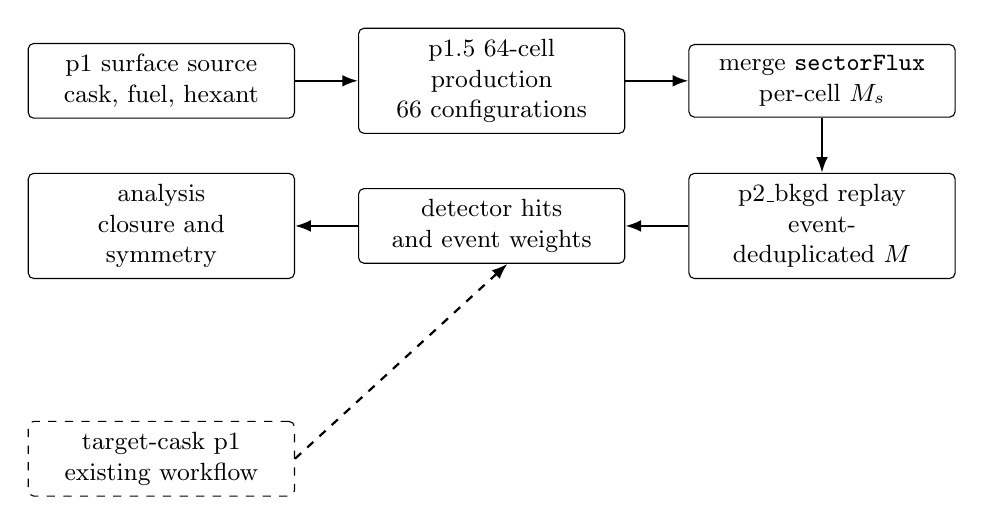
\begin{tikzpicture}[
      node distance=7mm and 8mm,
      box/.style={draw, rounded corners=2pt, align=center,
                  font=\small, inner sep=4pt, text width=3.1cm},
      arr/.style={-{Latex[length=2mm]}, thick}
    ]
    \node[box] (p1) {p1 surface source\\cask, fuel, hexant};
    \node[box, right=of p1] (p15) {p1.5 64-cell production\\66 configurations};
    \node[box, right=of p15] (merge) {merge \texttt{sectorFlux}\\per-cell $M_s$};
    \node[box, below=of merge] (p2) {p2\_bkgd replay\\event-deduplicated $M$};
    \node[box, left=of p2] (hits) {detector hits\\and event weights};
    \node[box, left=of hits] (ana) {analysis\\closure and symmetry};

    \draw[arr] (p1) -- (p15);
    \draw[arr] (p15) -- (merge);
    \draw[arr] (merge) -- (p2);
    \draw[arr] (p2) -- (hits);
    \draw[arr] (hits) -- (ana);

    \node[box, below=18mm of ana, dashed] (target) {target-cask p1\\existing workflow};
    \draw[arr, dashed] (target.east) -- ([xshift=2mm]hits.south);
  \end{tikzpicture}
  \caption{Two-stage background workflow. The p1.5 stage performs the expensive
  cask-to-cell transport once per source configuration; the p2\_bkgd stage
  reuses the unit-weight phase space for detector and shield variants. The
  dashed path is the existing target-cask workflow.}
  \label{fig:workflow}
\end{figure}

\section{Fast \SI{662}{keV} gamma validation}
\label{sec:gamma-validation}

\subsection{Configuration and direct reference}

The validation uses the \SI{662}{keV} gamma line from global fuel 0 of cask 4,
the assembly nearest to the nominal detector. The detector is the full nominal
CLYC assembly: crystal, casing, photomultiplier, \SI{50}{mm} lead collimator,
\SI{50}{mm} polyethylene collimator, and the polyethylene plug lip. The LiF
collimator is disabled. The detector is at
$(x,y,z)=(\SI{2930}{mm},\SI{1580}{mm},\SI{150}{mm})$ with rotation
$(0,-90,0)^\circ$ in the nominal macro.

The direct ZLN file for cask 4 and global fuel 0 contains 5016 detector hits and
a total deposited energy of \SI{1048.78}{MeV} for a \SI{180}{s} exposure.
Scaling linearly to the \SI{36}{s} exposure used here gives an expectation of
1003.2 hits and \SI{209.756}{MeV}. The comparison is a closure test of the
factorised workflow against a direct full-geometry calculation, not a new
measurement.

The full gamma source contains \num{350820506} surface crossings in
\SI{23}{GB}, so loading it whole would exceed the workstation memory. The
validation therefore uses a random one-million-event subset drawn from the
$10^8$-event source. The subset contains \num{3484873} crossings with total
weight \num{0.0129822}. With \num{1000000} source events and
$T_{\mathrm{gen}}=\SI{36}{s}$ the p1.5 normalisation gives
\begin{equation}
  N_{p1.5} =
  (36~\mathrm{s})(1.4\times10^{14}~\mathrm{s^{-1}})
  \frac{0.0129822}{10^6}
  = 6.543\times10^7
\end{equation}
source events. The run uses eight threads and no biasing. The output file is
written only after the event loop finishes; a partial file is not a valid
source. The \SI{36}{s} exposure is written as two independent \SI{18}{s}
chunks, \texttt{p15\_gamma662\_cask4\_1Mevt\_18s\_z8\_a.root} and
\texttt{\_b.root}. A single \SI{36}{s} file reached \SI{2.7}{GB} and its ROOT
key directory was unreadable; each \SI{18}{s} chunk remains at about
\SI{1.4}{GB}. Each chunk carries its own \texttt{sectorMeta} row with
$T_{\mathrm{gen}}=\SI{18}{s}$; the p2 replays are run per chunk and summed.

\subsection{p1.5 output and cell population}

The two \SI{18}{s} p1.5 chunks together produced \num{65430160} generated
events, \num{32715080} per chunk. Each \texttt{sectorMeta} row records
\texttt{nSectors}=8, \texttt{nZLayers}=8, \texttt{nCells}=64,
\texttt{zMin}=\SI{-2040}{mm}, \texttt{zMax}=\SI{2040}{mm},
and \texttt{dz}=\SI{510}{mm}. Each \texttt{sectorFlux} tree contains one entry
for each first crossing of a gamma into a cell. The entries are not spread
uniformly over the 64 cells: the source assembly illuminates the cells that face
it, and the azimuthal side entries are concentrated in the sectors adjacent to
that direction.

Figure~\ref{fig:map} shows the cask-local $x$--$y$ entry map and the
outer-face $z$--$\phi$ map for the first \SI{18}{s} chunk, and
Figure~\ref{fig:dist} shows the cell population, face label, kinetic energy,
longitudinal position, radial position, and polar angle.
The second chunk has the same layout and is not plotted separately. The energy distribution
is narrow because the source is a single gamma line plus the p1 smearing. The
radial distribution fills the shell between the inner and outer radii, with the
expected concentration near the inner surface. The longitudinal distribution
shows that the full-height shell is populated at both ends; the entries near
the cask top and bottom are real first crossings, not an artefact of a truncated
scoring surface.

\begin{figure}[t]
  \centering
  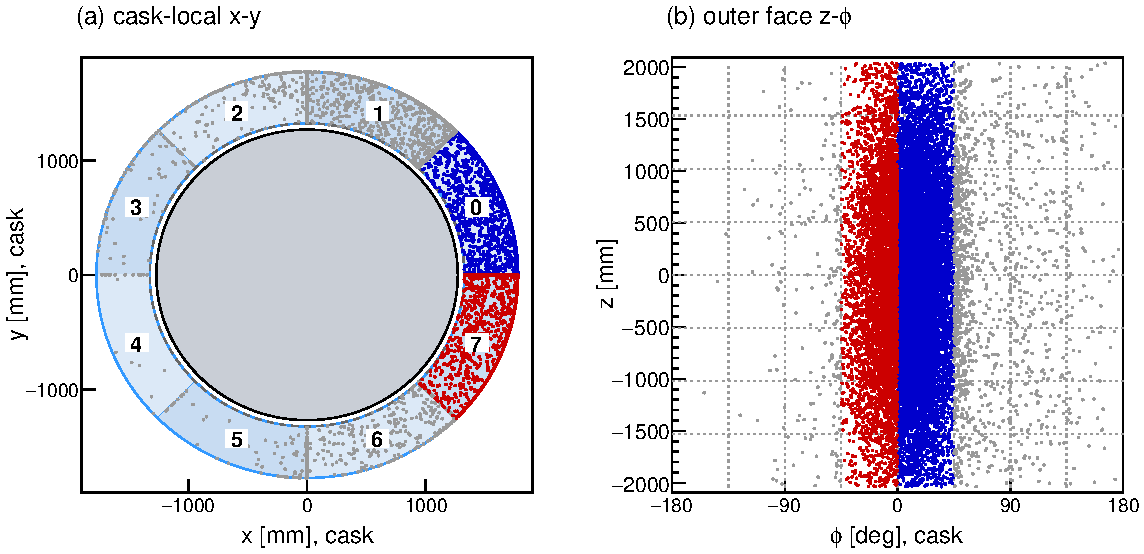
\includegraphics[width=\linewidth]{fig_p15_map.pdf}
  \caption{First-entry maps for the first \SI{18}{s} chunk of the 64-cell p1.5
  source. Left: cask-local $x$--$y$ map, showing the eight sectors. Right:
  longitudinal position $z$ versus azimuth $\phi$ for entries on the outer
  cylindrical face. The cell identifier is
  $\texttt{zLayer}\times 8+\texttt{sector}$. The source is one fuel assembly of
  cask 4, so the entries are localised in azimuth and in the longitudinal layer
  that faces the assembly. The blue and red entries mark sectors 0 and 7, the
  two sectors that contain the detector envelope. The left map uses a
  \num{10000}-entry subsample and the right map a \num{30000}-entry subsample
  for legibility; the histograms use all entries.}
  \label{fig:map}
\end{figure}

\begin{figure}[t]
  \centering
  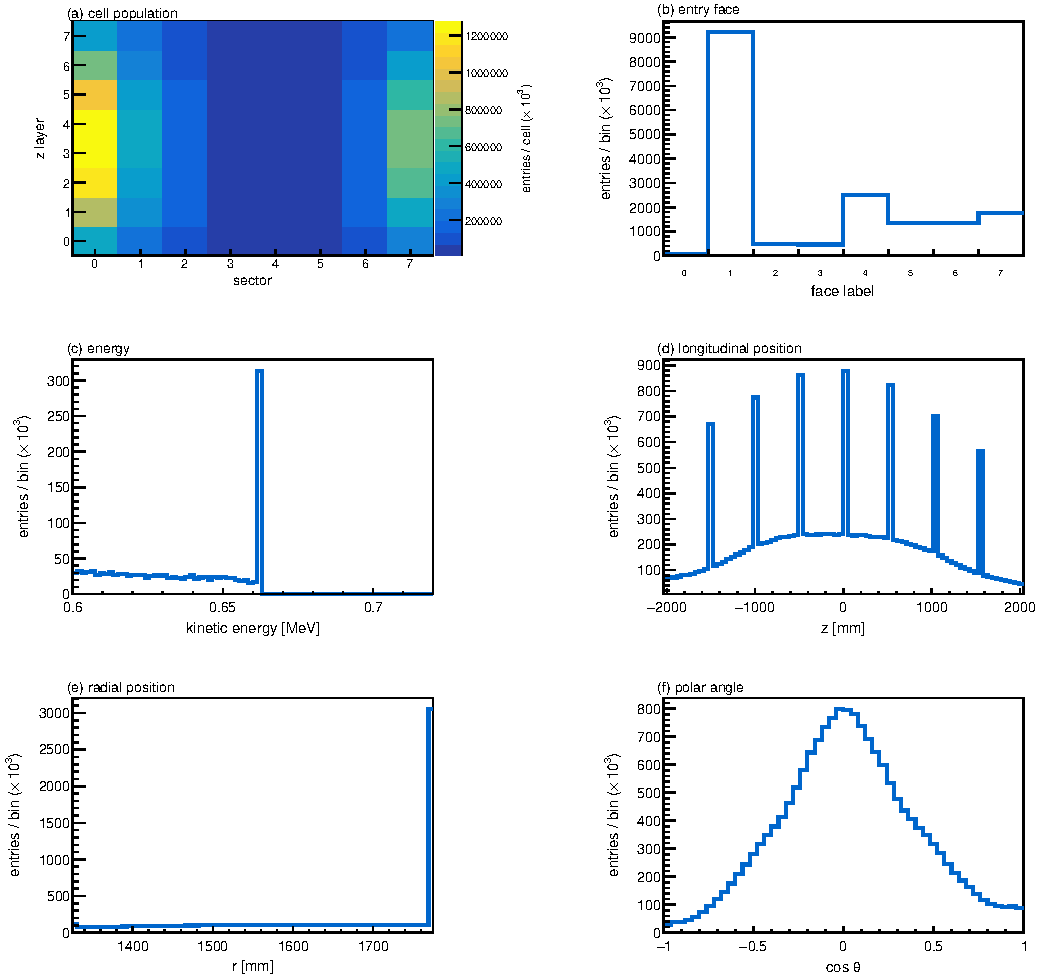
\includegraphics[width=\linewidth]{fig_p15_dist.pdf}
  \caption{p1.5 \texttt{sectorFlux} distributions for the first \SI{18}{s}
  chunk: cell population, entry face, kinetic energy, longitudinal position,
  radial position, and polar angle. Face labels 0--5 are the external inner,
  outer, top, bottom, and two azimuthal surfaces; labels 6 and 7 are the internal
  longitudinal boundaries between layers.}
  \label{fig:dist}
\end{figure}

\subsection{Replay result}

The automatic cell selection returns cells 32 and 39. The replay loaded
\num{3936600} entries for these cells and retained \num{3806673} unique source
events after deduplication, so \num{129927} entries were removed as repeated
crossings of the same event. With $T_{\mathrm{replay}}=T_{\mathrm{gen}}$,
Equation~\eqref{eq:replay} gives \num{3806673} generated primaries. The replay
produced 961 detector hits and a total deposited energy of \SI{208.740}{MeV}.

A second replay used four cells, 24, 31, 32, and 39, to test whether the layer
below the detector contributes a significant flux. It loaded \num{7964658}
entries, retained \num{6846190} unique events, and generated \num{6846190}
primaries. It produced 1016 hits and \SI{212.392}{MeV}. The additional layer
therefore changes the hit count by 5.7\% and the deposited energy by 1.7\%,
which is consistent with the detector envelope being confined to layer 4 and
with the small number of entries in the adjacent layer.

Table~\ref{tab:gamma-validation} compares the two replay results with the direct
ZLN expectation. The two-cell replay gives a hit ratio of 0.958 and an energy
ratio of 0.995. The four-cell replay gives 1.013 and 1.013. The two-cell sample
contains about 953 independent hit events, so the statistical uncertainty on the
hit count is approximately 3.2\%. The two-cell and four-cell results bracket the
direct yield; their difference is about 1.2 standard deviations and is
therefore not significant at this sample size. They are not precise enough to exclude a
few-percent bias, but they exclude a 10\% normalisation error.

The 64-cell background model therefore reproduces the direct ZLN yield at the
3\% statistical level for this configuration. The remaining difference is
within the statistical uncertainty of this sample; a larger replay is needed to
test for a few-percent bias.

\begin{table}[H]
  \centering
  \caption{\SI{662}{keV} gamma validation for cask 4 / global fuel 0. The direct
  ZLN yield is scaled from \SI{180}{s} to the \SI{36}{s} exposure. The p2 entry
  counts are the p1.5 entries after the cell filter and before and after
  event-level deduplication.}
  \label{tab:gamma-validation}
  \begin{tabular}{lrrrrr}
    \toprule
    Replay & $M_{\mathrm{loaded}}$ & $M_{\mathrm{unique}}$ &
    $N_{\mathrm{replay}}$ & Hits & Deposited energy [MeV] \\
    \midrule
    Direct ZLN, scaled to \SI{36}{s} & --- & --- & --- & 1003.2 & 209.756 \\
    p2, cells 32 and 39 & \num{3936600} & \num{3806673} & \num{3806673} & 961 & 208.740 \\
    p2, cells 24, 31, 32, 39 & \num{7964658} & \num{6846190} & \num{6846190} & 1016 & 212.392 \\
    \bottomrule
  \end{tabular}
\end{table}

Figure~\ref{fig:gamma-models} shows the corresponding energy-deposition
spectra and the bin-by-bin ratio to the direct ZLN result.

\begin{figure}[H]
  \centering
  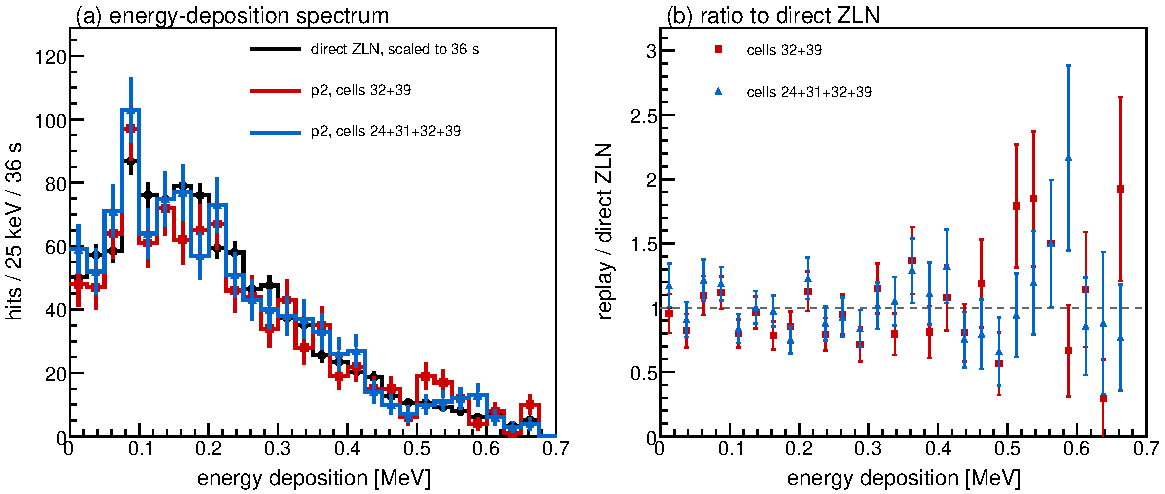
\includegraphics[width=\linewidth]{fig_gamma_models.pdf}
  \caption{Energy-deposition spectra for the direct ZLN gamma-662 run and the
  64-cell replay. The left panel shows absolute counts per \SI{25}{keV} bin
  scaled to the \SI{36}{s} exposure; the right panel shows the ratio of the
  replay to the direct ZLN spectrum. The replays are event-deduplicated. The
  two-cell selection uses the cells that contain the detector envelope; the
  four-cell selection adds the layer below it as a systematic check.}
  \label{fig:gamma-models}
\end{figure}

\subsection{What the validation does and does not show}

The validation shows that the 64-cell shell is populated, that the cell and face
identifiers are written correctly, that the metadata row records the 64-cell
layout, that the automatic cell selection returns the two cells that contain the
nominal detector, and that the event-deduplicated replay produces a detector
signal close to the direct ZLN result. It does not provide a background
estimate. The source is one gamma line from one fuel assembly, the p1 file is a
one-million-event subset, the detector is a single CLYC at one position, and the
replay uses one candidate entry per source event. The 961-hit sample, with 953
independent hit events, has a 3.2\% statistical uncertainty on the hit count; it
is sufficient to exclude a 10\% normalisation error but not to constrain the
spectral shape at the few-percent level.

\section{HPC production and validation plan}

\subsection{Production matrix}

The target cask is cask 0. The other eleven casks are background sources, and
each source cask is combined with six hexants. This gives
\begin{equation}
  11\ \text{casks}\times 6\ \text{hexants}=66
\end{equation}
independent p1.5 production configurations. The target cask remains passive in
all of them. Table~\ref{tab:matrix} groups the runs by cluster.

\begin{table}[H]
  \centering
  \caption{p1.5 production matrix. Each row is multiplied by six hexants.}
  \label{tab:matrix}
  \begin{tabular}{@{}lcc@{}}
    \toprule
    Source group & Background casks & p1.5 runs \\
    \midrule
    Central cluster & 3 & 18 \\
    $+x$ cluster & 4 & 24 \\
    $-x$ cluster & 4 & 24 \\
    \midrule
    Total & 11 & 66 \\
    \bottomrule
  \end{tabular}
\end{table}

The runs are embarrassingly parallel: each configuration reads the same p1
file, builds the same cask array, and writes its own \texttt{sectorFlux} and
\texttt{sectorMeta} output. A job array with one element per
\texttt{(cask, hexant)} pair is the natural mapping. The production macro must
remove the one-million-event subset, use the full p1 source, and use the
production $T_{\mathrm{gen}}$. The target cask must be present in the geometry
even when it is not the source, because the scoring shell is centred on it.

\subsection{Cost model and HPC requirement}

Let $C_{\mathrm{cfg}}$ be the measured wall-clock cost of one p1.5
configuration and $N_{\mathrm{cfg}}=66$. The production cost is
\begin{equation}
  C_{\mathrm{prod}} = 66\,C_{\mathrm{cfg}}
\end{equation}
before accounting for queueing and failed-job resubmission. The replay stage
adds
\begin{equation}
  C_{\mathrm{replay}} = N_{\mathrm{scan}}\,C_{\mathrm{scan}},
\end{equation}
where a scan is one \texttt{(cell selection, detector, shield)} combination. The
replay is cheaper per event than p1.5 because it starts from a unit-weight
phase-space entry and does not repeat the cask-to-cell transport, but it is not
free: the number of replayed primaries from Equation~\eqref{eq:replay} can be
large.

The measured 64-cell p1.5 rate on this eight-core workstation is about
\SI{15000}{evt/s} for the \SI{662}{keV} gamma source, so one \SI{36}{s}
configuration with $6.543\times10^7$ events takes about \SI{73}{min}. The
corresponding replay of $3.8\times10^6$ primaries takes a few minutes. These
rates scale with the source type and the number of secondary particles; the
neutron case is slower per event. The production campaign is therefore an
HPC-scale workload, and the 66 independent p1.5 jobs map naturally to a job
array. A workstation can produce a single validation configuration but should
not serialise the full matrix.

\subsection{Neutron validation plan}

For neutrons, the closure test is more expensive but remains the
production-relevant check. The same cask 4 / global fuel 0 configuration is the
natural choice: cask 4 is at $(x,y)=(\SI{6240}{mm},\SI{1580}{mm})$, and its
fuel-0 centre is at $(-662,+127)$~mm in the cask frame, i.e. on the
detector-facing side. The direct ZLN file contains 1063 detector hits for
\SI{180}{s}, so it provides the requested $\mathcal{O}(10^3)$ count level.

The neutron p1.5 run has not yet been repeated with the 64-cell shell. The
production validation must use the same cell selection and event
deduplication as the gamma case, and it must record the number of entries on the
two azimuthal side faces and on the internal longitudinal boundaries. Folding
side entries into the radial faces would bias the face-resolved comparison. The
replay must sample the cells that contain the detector; for the nominal position
these are the sector-0 and sector-7 cells of layer 4.

\subsection{Merging and metadata}

The merger must preserve the per-cell entry count. A production file may
contain one metadata row per cell, or the merger may add an explicit
\texttt{M\_cell} count alongside the existing total $M$. The replay sampler
filters on \texttt{cellId} and computes $M_{\mathrm{loaded}}$ and
$M_{\mathrm{unique}}$ from the filtered entries, so the physics normalisation is
correct even if the metadata stores only the total; the per-cell count is still
needed for bookkeeping and for detecting missing or duplicated files.

The merger should also check that the 64 cell identifiers are present or
accounted for, that the shell dimensions and the number of longitudinal layers
agree across files, that the target cask is the same in every file, and that no
file was produced with a different p1 source or smearing configuration. The
source cask, source type, hexant, global fuel, and batch identifier are already
stored per entry and in the metadata.

\subsection{Validation checklist}

The following checks should be completed before the production result is used:

\begin{enumerate}
  \item \textbf{Geometry containment.} Verify that the detector and shield lie
        between the inner and outer faces, do not overlap the cask body, and
        that the hemi-shield variant remains inside the shell and clear of the
        inner face. For the nominal detector at $\varphi=0^\circ$, note that it
        lies on the boundary between sectors 0 and 7; both cells must be
        selected.
  \item \textbf{Cell coverage.} Verify that every populated cell has a non-zero
        entry count, that the cell identifiers are unique, and that the sum of
        the per-cell counts equals the total entry count. Check the two
        external caps and the internal longitudinal labels separately.
  \item \textbf{First-entry correctness.} Compare the number of entries with
        and without the boundary-status check and with a step-level reference
        count; confirm that the 256-bit mask suppresses duplicates without
        killing tracks.
  \item \textbf{Deduplication.} Compare the event-deduplicated replay with a
        track-aware replay for the same source sample. The difference measures
        the bias introduced by keeping only the earliest entry per event. At
        minimum, report $M_{\mathrm{loaded}}$, $M_{\mathrm{unique}}$, and the
        fraction removed for every cell selection.
  \item \textbf{Phase-space closure.} Repeat the p1.5-to-p2 closure test for
        every populated cell and for both particle types. Check energy, polar
        angle, azimuth, and all face categories.
  \item \textbf{Symmetry.} Rotate a source configuration by \ang{60} (hexant)
        or \ang{45} (sector) and compare the cell populations after the
        corresponding rotation. Deviations should be consistent with the
        geometry, not with a bookkeeping error.
  \item \textbf{Normalisation.} Verify Equation~\eqref{eq:replay} against a
        direct p2 run for the same source and time. The ratio of hit yields
        should be consistent with one within statistics. Report the
        deduplication prescription and the selected cells with every ratio.
  \item \textbf{Reproducibility.} Record the executable commit, the p1 file
        checksum, the macro, the random seed, and the production
        $T_{\mathrm{gen}}$ for every output file.
\end{enumerate}

\section{Limitations and next steps}
\label{sec:limits}

The main limitations of the pilot are the single gamma line, the single source
cask, the one-million-event source subset, the single detector position, and the
event-level deduplication. The production campaign must address all of these. In
addition, the current metadata stores the total $M$; the merger should add the
per-cell count before the production files are archived. The gamma validation
used a one-million-event random subset because the full source exceeds the
workstation memory; the subset normalisation is correct, but the full source
should be used in production.

The deduplication is the most important modelling approximation. It keeps the
earliest entry per source event, which removes repeated crossings of the
artificial cell boundaries but also discards every later entry of the same
event. If a later entry is closer to the detector, the replay misses it. The
present gamma test is consistent with the direct ZLN result at the approximately
3\% statistical level, but it cannot distinguish the two-cell and four-cell
selections, whose hit yields differ by 5.7\%. A track-aware replay, or a replay
that carries all cell entries with an explicit per-entry weight, is required
before the 64-cell phase space is used for a production background estimate.

The geometry near the inner radius also deserves a dedicated check. The sector
inner radius is close to the fin tips, and a detector or shield placed at the
nominal radius could, in some configurations, approach the inner face. The shell
is a parallel-world scoring surface, so an intersection would not change the
transport, but it would change the interpretation of the first-entry sample. The
containment check should be part of the production qualification.

Finally, the OpenGL renders in this report are illustrative. They omit the hall
and hide internal cask details. The dimensioned plan view and the
radial--longitudinal cross-section remain the reference figures for geometry.

\section{Conclusion}

The 64-cell background-sector workflow is implemented and exercised end to end.
The p1.5 stage scores first entries into a parallel-world shell of eight
azimuthal sectors and eight longitudinal layers, the p2\_bkgd stage replays the
unit-weight phase space through the detector geometry, and the \SI{662}{keV}
gamma check reproduces the direct ZLN yield at the approximately 3\% statistical
level. The event-level deduplication removes repeated crossings of the
artificial cell boundaries, but it keeps only one candidate entry per source
event; a track-aware replay is therefore required before the nominal detector
position is validated at the few-percent level. The production campaign requires 66
independent p1.5 configurations and a set of replay scans; this is an HPC-scale
workload, but it is embarrassingly parallel and can be mapped to a job array.
The next step is to remove the one-million-event subset, add per-cell metadata,
run the production matrix, and complete the validation checklist.

\appendix

\section{Reproducing the validation}

The p1.5 validation requires the background-sector mode on the command line
because the parallel world must be registered before the macro runs:
\begin{verbatim}
./build/G4DCSmonitor --mode background-sector \
  macros/validation/p15_gamma662_cask4_1Mevt_18s_a.mac
./build/G4DCSmonitor --mode background-sector \
  macros/validation/p15_gamma662_cask4_1Mevt_18s_b.mac
\end{verbatim}
The p2 replay uses the same executable without \texttt{-{}-mode}:
\begin{verbatim}
./build/G4DCSmonitor \
  macros/validation/p2_gamma662_cask4_1Mevt_18s_a.mac
./build/G4DCSmonitor \
  macros/validation/p2_gamma662_cask4_1Mevt_18s_b.mac
./build/G4DCSmonitor \
  macros/validation/p2_gamma662_cask4_1Mevt_18s_4cell_a.mac
./build/G4DCSmonitor \
  macros/validation/p2_gamma662_cask4_1Mevt_18s_4cell_b.mac
\end{verbatim}
The two 18~s p2 outputs are combined with \texttt{hadd}:
\begin{verbatim}
hadd -f build/validation/p2_gamma662_cask4_1Mevt_36s_z8.root \
  build/validation/p2_gamma662_cask4_1Mevt_18s_z8_a.root \
  build/validation/p2_gamma662_cask4_1Mevt_18s_z8_b.root
hadd -f build/validation/p2_gamma662_cask4_1Mevt_36s_4cell_z8.root \
  build/validation/p2_gamma662_cask4_1Mevt_18s_z8_4cell_a.root \
  build/validation/p2_gamma662_cask4_1Mevt_18s_z8_4cell_b.root
\end{verbatim}
The validation macros use cask 4 and global fuel 0, set the 64-cell layout with
the command
\begin{verbatim}
/dcs-monitor/det/setSectorZLayers 8
\end{verbatim}
and write files with the \texttt{\_z8} suffix. The source file is
\texttt{surface\_gamma662\_cask4\_1Mevt.root} in
\path{build/validation}. The figures are
generated from the repository root with
\begin{verbatim}
root -l -b -q report/sector_implementation/scripts/make_geometry_figs.C
root -l -b -q report/sector_implementation/scripts/make_data_figs.C
./report/sector_implementation/scripts/make_ogl_figs.sh
\end{verbatim}
The data figures use the first 18~s p1.5 chunk by default; set
\texttt{P15\_FILE} to another chunk to reproduce the maps from that file. The
ROOT scripts crop the PDF page boxes with \texttt{pdfcrop}; the OGL driver
exports vector PDFs and rasterises them for the report.

\end{document}
